\graphicspath{{chapters/_resources/}}

\chapter{Enhancer regulation}



\hypertarget{tcic-1}{%
\section{5 - TCiC (1)}\label{tcic-1}}

Enhancer regulation is controlled by specific transcription factors with a DBD. Most of the times, TFs interact with PIC through co-factors. In particular, the Mediator is a key co-activator complex of RNA pol II transcription regulation.

\hypertarget{mediator-complex}{%
\subsubsection{Mediator complex}\label{mediator-complex}}

The Mediator complex is a multi subunit complex, composed of almost 30 subunits. CDK8 is the only module with enzymatic activity.

\begin{figure}
\centering
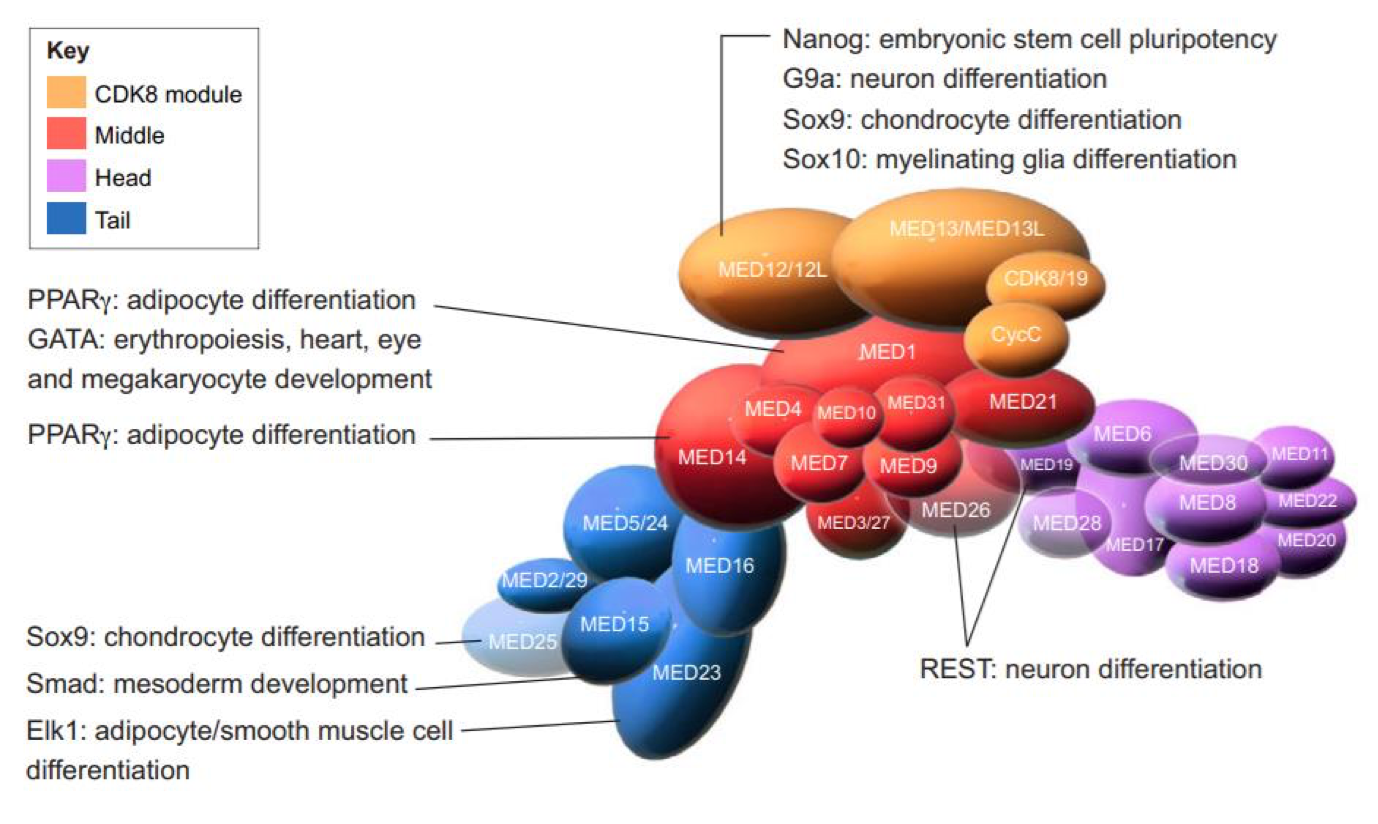
\includegraphics[width=0.5\textwidth]{../_resources/Screenshot_2022-10-07_at_10-47-50.png}
\caption{Screenshot 2022-10-07 at 10.47.50.png}
\end{figure}

The Mediator complex can interact with hundreds of TFs and integrate their function, allowing cooperation and regulation of multiple sites in enhancer regions. Examples: SOX,c-Myc,\ldots{}

Since the Mediator is a multi-subunit structure, a conformational change in one subunit propagates to the whole complex.

The interaction with Pol II prevents the catalytic interaction: the core mediator has mutually exclusive interactions.

\begin{figure}
\centering
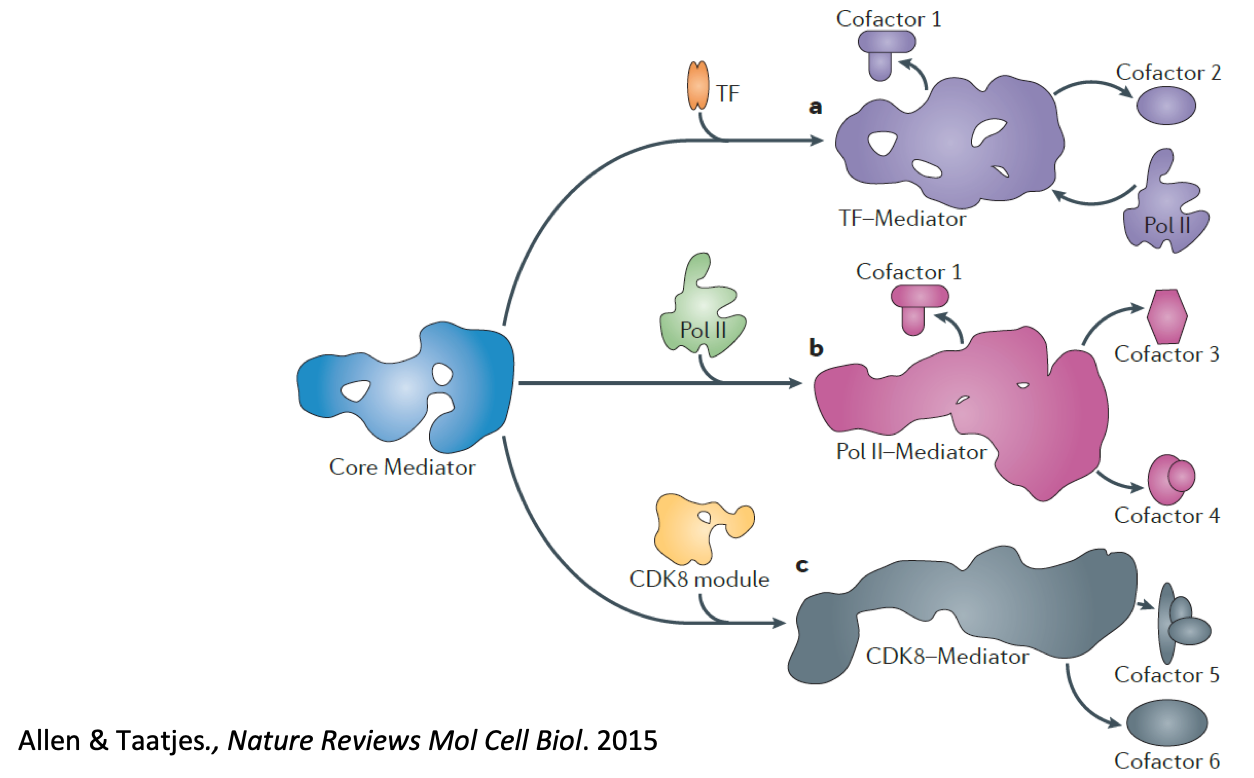
\includegraphics[width=0.5\textwidth]{../_resources/Screenshot_2022-10-07_at_10-50-30.png}
\caption{Screenshot 2022-10-07 at 10.50.30.png}
\end{figure}

The Mediator functions as a bridge between the TFs bound to the enhancers and the PIC at core promoters; DNA looping involves \emph{cohesins} (circle DNA). The interaction with enhancers occurs first and is more stable than the core promoter one.

\begin{figure}
\centering
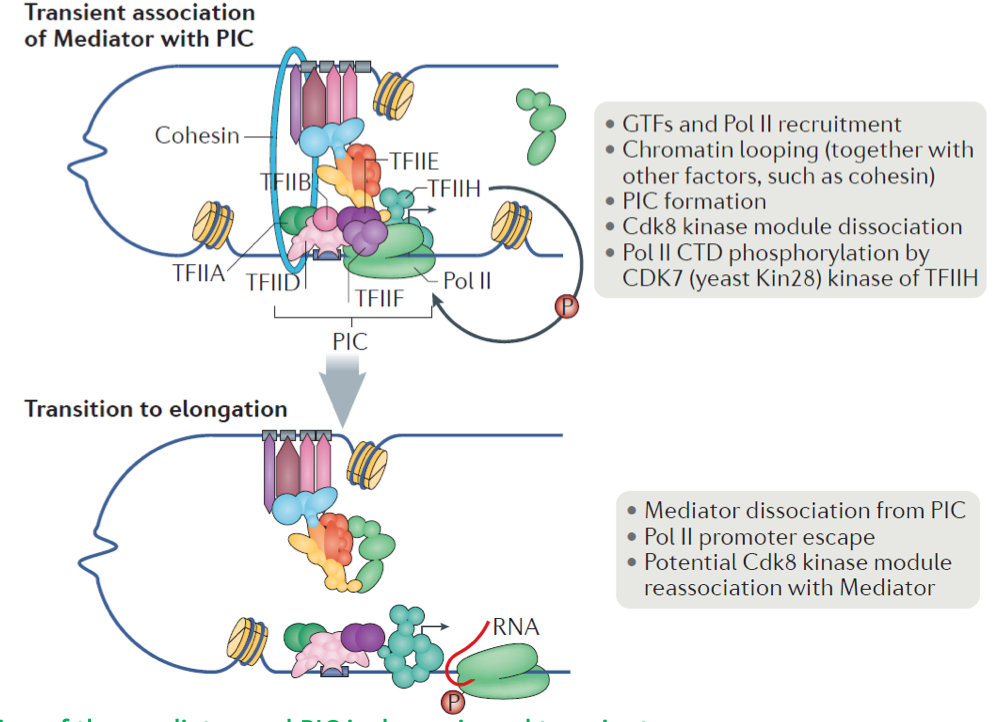
\includegraphics[width=0.5\textwidth]{../_resources/Screenshot_2022-10-07_at_10-54-13.png}
\caption{Soutourina\emph{, Nature Review Mol Cell Biol.} 2018}
\end{figure}

Soutourina\emph{, Nature Review Mol Cell Biol.} 2018

The Mediator stimulates transcription at several levels: assembly of the PIC, chromatin organization, transcription elongation, nucleosome displacement at TATA-box promoters. After Pol II promoter escapes, the Mediator interacts with Cdk8 to activate pause release. The Mediator presence at TATA regions inversely correlates with nucleosome occupancy : indeed, it is able to bind acetylated histones and interact with chromatin remodelling complexes contributing in histone eviction.

The Mediator has been defined as GTF (general TF), however it preferentially associates with enhancers and its occupancy at core promoters is generally low and transient.

Once the Mediator is interacting with the PIC, CDK8 is displaced; afterwords, the Mediator is able to recruit it again to activate Cdk9, allowing the pausing mechanism.

\begin{figure}
\centering
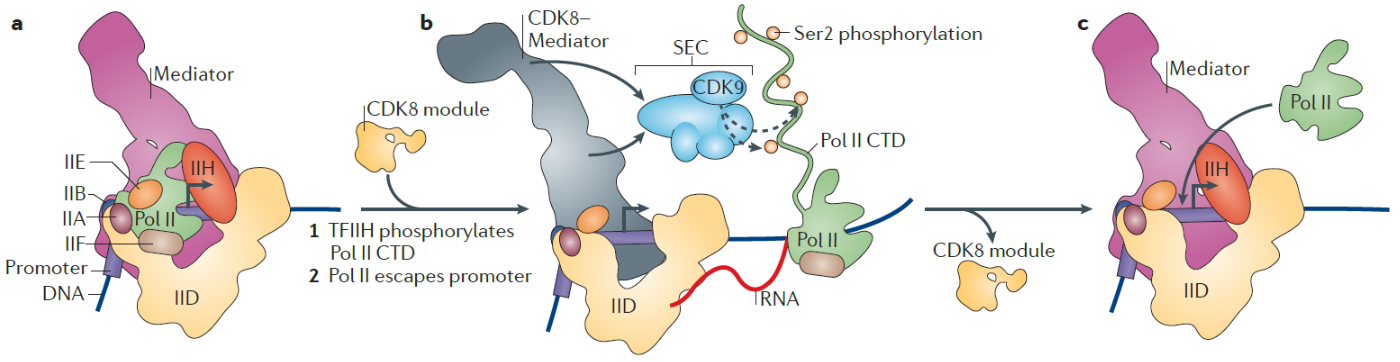
\includegraphics[width=0.5\textwidth]{../_resources/Screenshot_2022-10-10_at_11-03-13.png}
\caption{Allen and Taatjes, \emph{Nature Reviews Mol Cell Biol}. 2015}
\end{figure}

Allen and Taatjes, \emph{Nature Reviews Mol Cell Biol}. 2015

The multi-subunit and modular structure of the Mediator enables to respond to multiple signalling cascades activating transcription. Different subunits can be engaged in PPIs; we are interested in many of them, in particular oncogenes usually interact with the mediator.

\hypertarget{wnt-signalling-pathway}{%
\subsection{Wnt signalling pathway}\label{wnt-signalling-pathway}}

Wnt signalling pathway is a relevant pathway for morphogenesis and embryonic development, as well as adult tissue homeostasis. Its activation is associated with cell proliferation and cell renewal.

The pathway occurs at a plasma membrane, where \textasciitilde20 ligands interact among themselves and with a core receptor (either LRP5 or LRP6). A

\begin{itemize}
\tightlist
\item
  Off: XIN1 forms a \emph{destruction complex} with APC, CK1, GSK, which recruits \textbf{$\beta$  -catenin}, a relevant co-activator. The activation is performed through phosphorylation or ser and threonine residues, which will then recruit btrCP ubiquitinylase and lead to b-cat degradation.
\item
  On: when Wnt is present, the complex is sequestered and therefore b-catenin is not phosphorylated and ubiquitinylated, it remains present in the cell. Among target genes, AXIN2 promotes the recruitment and formation of distraction complex, others are plasma membrane proteins which promote \emph{endosome mediated degradation} of WNT.
\end{itemize}

\begin{figure}
\centering
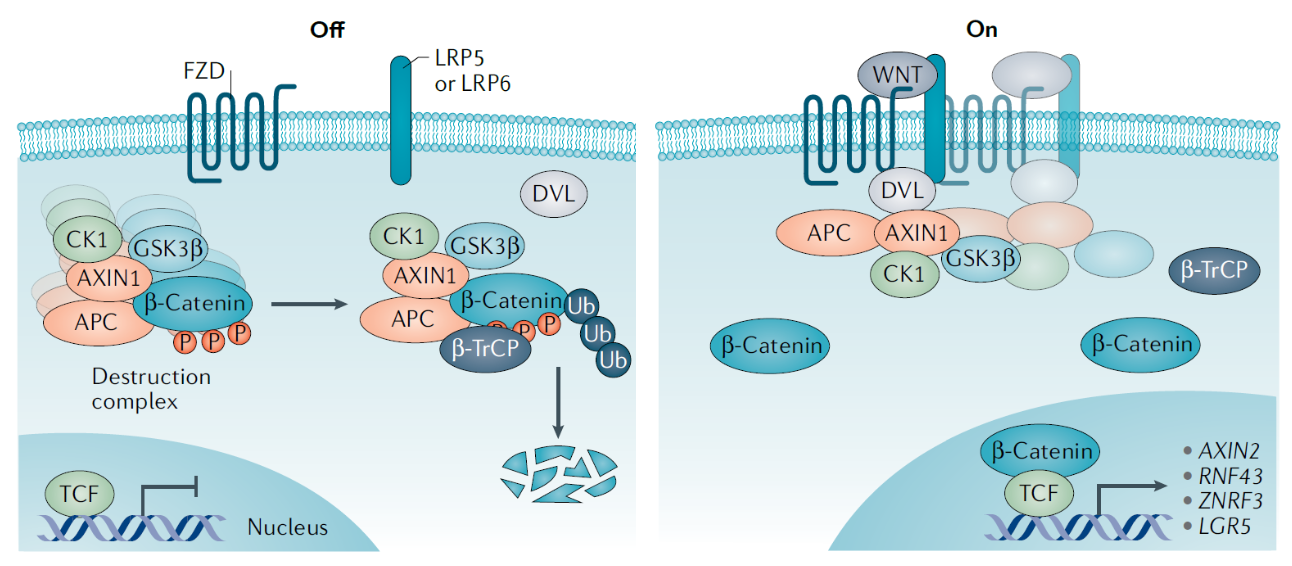
\includegraphics[width=0.5\textwidth]{../_resources/Screenshot_2022-10-10_at_11-03-55.png}
\caption{Bugter \emph{et al., Nature Review Cancer}, 2021}
\end{figure}

Bugter \emph{et al., Nature Review Cancer}, 2021

\begin{figure}
\centering
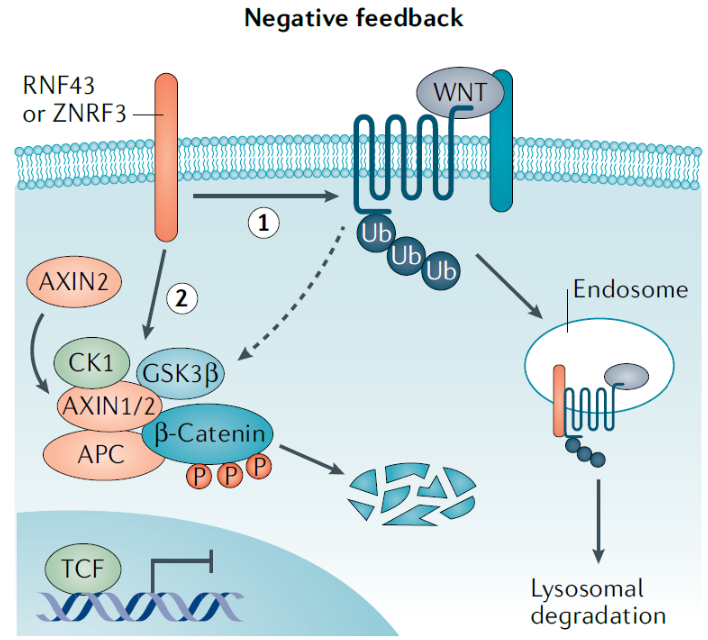
\includegraphics[width=0.5\textwidth]{../_resources/Screenshot_2022-10-10_at_11-04-14.png}
\caption{Screenshot 2022-10-10 at 11.04.14.png}
\end{figure}

Wnt is synthesized in the endoplastic reticulum, lipid modified and released from cells through EVs (or can remain attached to membrane of secreting neighbouring cells). It can spread and reach different sites.

Excessive $\beta$  -catenin activity in cancer can occur due to:

\begin{itemize}
\tightlist
\item
  inactivating mutations in members of the destruction complex
\item
  negative feedback pathway (RNF43 or ZNRF3) and activating mutations $\beta$  -catenin
\end{itemize}

Genetic alterations in the WNT pathway occur in most cancer types with some components of the pathway showing tissue specificity. All WNT mutations converge in enhancing $\beta$  -catenin activity, although with different extent, and cooperate with other driver mutations to promote tumorigenesis. Mutation are considered early (APC) or late (RNF43) events and associate with different tumor subtypes. APC mutant tumor leads to many clinical features: depending on the function and position in the pathway of the gene, the downstream effect can be very different.

In absence of $\beta$  -catenin (Wnt pathway off), TLE and HDAC bind TCF and stop transcription. $\beta$  -catenin subcellular translocation is presumed to function thanks to the binding of adaptor proteins. $\beta$  -catenin needs to interact with different TFs, among which TCF family members are the most common and expressed in different forms. They all recognize the same binding site. In particular, different isoforms of TCF7 and LEF1 are highly expressed in colorectal cancer.

\hypertarget{ux3b2-catenin-structure}{%
\subsubsection{$\beta$  -catenin structure}\label{ux3b2-catenin-structure}}

$\beta$  -catenin structure acts as a binding platform for numerous interactions. It is composed of 781 aa residues in humans and divided in:

\begin{itemize}
\tightlist
\item
  central highly repetitive sequence with \emph{Armadillo sequence} important for nuclear activity.
\item
  Helix-C conserved structure close to CTD
\item
  C-terminal transcription activator domain (CTTA)
\end{itemize}

Key interactors: E-cadherin and A-cathenin → structural function, focal adhesion. Decrease in E-cadherin is found in EMT. E-cadherin cad is stabilized by $\beta$  -catenin, therefore with low levels of $\beta$  -catenin we observe an E-cadherin decrease in ETM.

The function of $\beta$  -catenin, both structural and signaling, is regulated by post-translational modifications.

RNA pol II is also loaded on inactive genes; to foster elongation we require $\beta$  -catenin, which can recruit PAF1 complex. The majority interact with the CTTA domain, which serves as a binding platform or trans-activation domain.

\begin{figure}
\centering
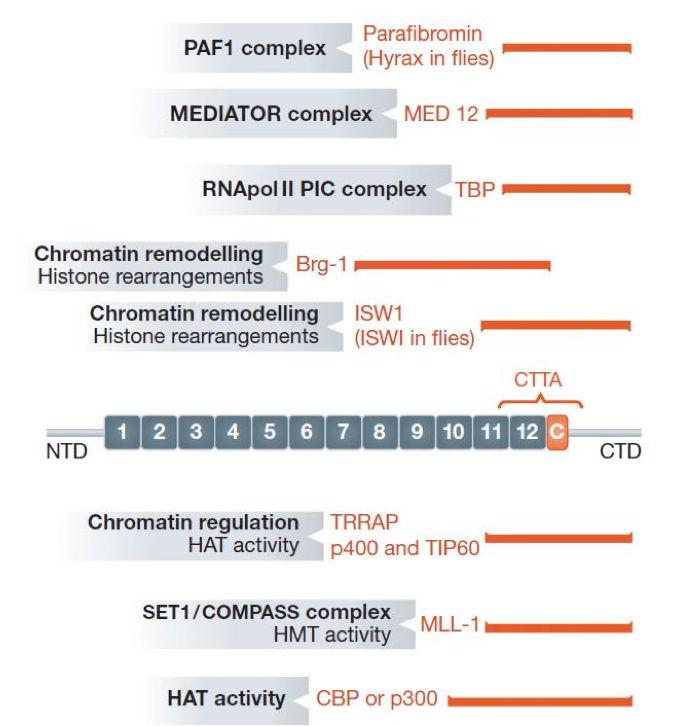
\includegraphics[width=0.5\textwidth]{../_resources/Screenshot_2022-10-07_at_11-52-13.png}
\caption{Valenta \emph{et al., EMBO J.} 2012}
\end{figure}

Valenta \emph{et al., EMBO J.} 2012

\begin{figure}
\centering
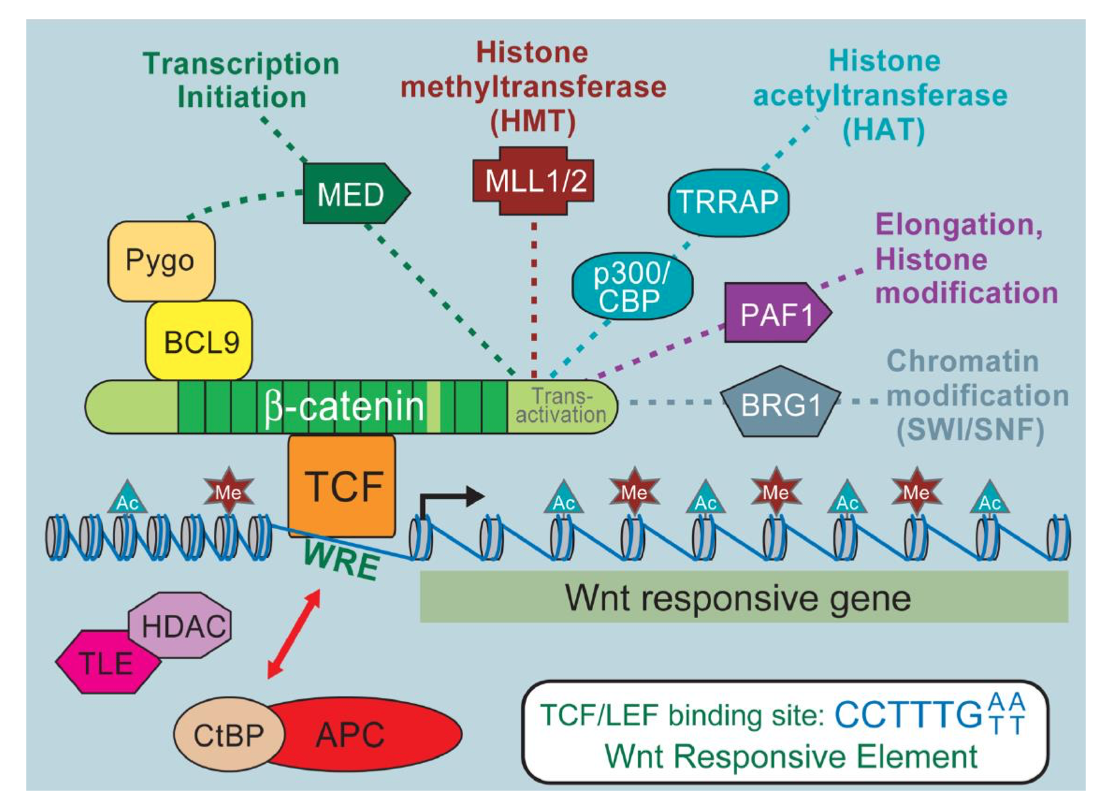
\includegraphics[width=0.5\textwidth]{../_resources/Screenshot_2022-10-07_at_11-52-58.png}
\caption{McDonald \emph{et al., Dev Cell}, 2009}
\end{figure}

McDonald \emph{et al., Dev Cell}, 2009

\hypertarget{the-canonical-wntux3b2-catenin-pathway-is-crucially-involved-in-colorectal-cancer}{%
\subsubsection{\texorpdfstring{\textbf{The canonical Wnt/$\beta$  -catenin pathway is crucially involved in colorectal cancer}}{The canonical Wnt/$\beta$  -catenin pathway is crucially involved in colorectal cancer}}\label{the-canonical-wntux3b2-catenin-pathway-is-crucially-involved-in-colorectal-cancer}}

The \textbf{APC gene} was first identified by being mutated in a hereditary colon cancer syndrome termed familiar adenomatous polyposis. Most cases of sporadic colorectal cancer result from loss of both APC alleles. Loss of APC function leads to the inappropriate stabilization of $\beta$  -catenin and the formation of constitutive complexes between $\beta$  -catenin and the intestinal TCF family member TCF7l2/TCF4 Patients with hereditary Axin2 mutations display a predisposition to colon cancer. Aberrant activation of the canonical Wnt/$\beta$  -catenin pathway occurs in almost all colorectal cancers, contributing to their growth, invasion and survival.

\emph{Luciferase reporter genes}: firefly and renilla Luc, of the two only one has a responsive site to TCF. It is a control for the efficiency of transfection.

Let's see which genes are involved in the regulation of $\beta$  -catenin through RNAi in DLD1 cells: 34 genes are necessary for $\beta$  -catenin activity and 166 candidate genes are necessary for HCT116 cells proliferation. By merging the two groups, we can identify a set of 9 potential regulators of colon cancer proliferation and $\beta$  -catenin activity: CDK8, CSK1G3, CSNK1E, DKC1, MAP3K14, MLLT7, PLK4, TAOK1 and ZAK.

Genome wide analysis of chromosome copy number alterations (CNA) in human CRC biopsies revealed amplification of chr. 13 region including CDK8. Immunohistochemical analysis of CDK8 expression in the same 50 specimens revealed elevated protein levels in 26\% colon cancer samples, including those that showed CDK8 CN gain {[}the brownish colour in IHC indicates that CDK8 expression increases{]}.

\begin{figure}
\centering
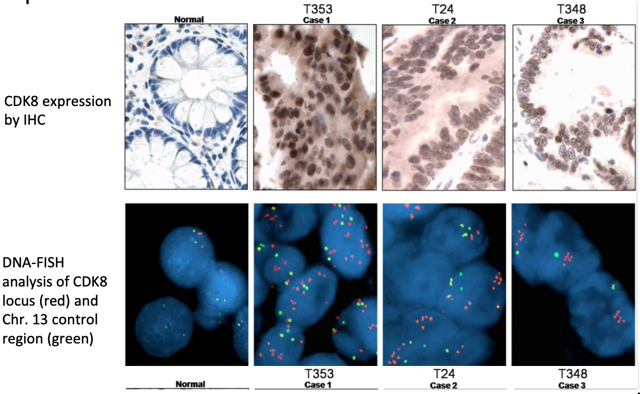
\includegraphics[width=0.5\textwidth]{../_resources/Screenshot_2022-10-10_at_12-23-14.png}
\caption{Firestein \emph{et al., Nature} 2008}
\end{figure}

Firestein \emph{et al., Nature} 2008

These observations indicate that CDK8 is amplified and overexpressed in a substantial fraction of colon cancers. In particular, CDK8 action is not a passenger effect, it is a \emph{driving proliferation}. There is a huge difference from in vitro and in vivo tumor setting: in order to obtain more suitable experiments, we can look at the transforming potential (as not all proliferating cells are necessarily tumor cells). If we combine $\beta$  -catenin in catalytically dead CDK8 we drop the affect, but it is not completely abolished - as $\beta$  -catenin can bypass the need engaging interactions with others.

\textbf{Main conclusions of the article}

\begin{itemize}
\tightlist
\item
  CDK8 acts as an oncogene in a substantial fraction of colorectal cancers
\item
  CDK8 kinase activity is essential to regulate $\beta$  -catenin dependent transcription and transformation
\item
  CDK8 acts in part by co-activating $\beta$  -catenin driven transcription in colon cancer with high CDK8 expression and $\beta$  -catenin activity
\end{itemize}

\underline{Therapeutic interventions that target CDK8 kinase activity may be of clinical value in colorectal cancer}

Almost all Mediator subunits have been found to be mutated/deregulated in a huge list of cancers e.g.~MED12 subunit in prostate cancer.

\hypertarget{transcriptional-control-in-cancer}{%
\section{6- Transcriptional Control in Cancer}\label{transcriptional-control-in-cancer}}

\href{https://www.notion.so/TCiC-08701b51973a4b22a16e226a1fbd7e9b}{TCiC}

\hypertarget{crepp300}{%
\section{CREP/p300}\label{crepp300}}

CREB-binding protein (CBP) and p300 is a heavily regulated TF. Differently from the Mediator, it is a monomer and has several trans-activation domain, which enable it to interact with TF and PIC. It has histone acetyltransferase activity (HAT) or lysine acetyltransferase activity (KAT). Chromatin will be modified by increasing accessibility and also TF regulation.

\hypertarget{crepp300-structure}{%
\subsubsection{CREP/p300 structure}\label{crepp300-structure}}

\begin{itemize}
\item
  4 transactivation domains
\item
  histidine rich or glutamine rich regions.
\item
  Zinc fingers domain for PPIs
\item
  bromodomain and PHD interact with histones
\item
  lysine acetyltransferase domain (HAT)

  \begin{figure}
  \centering
  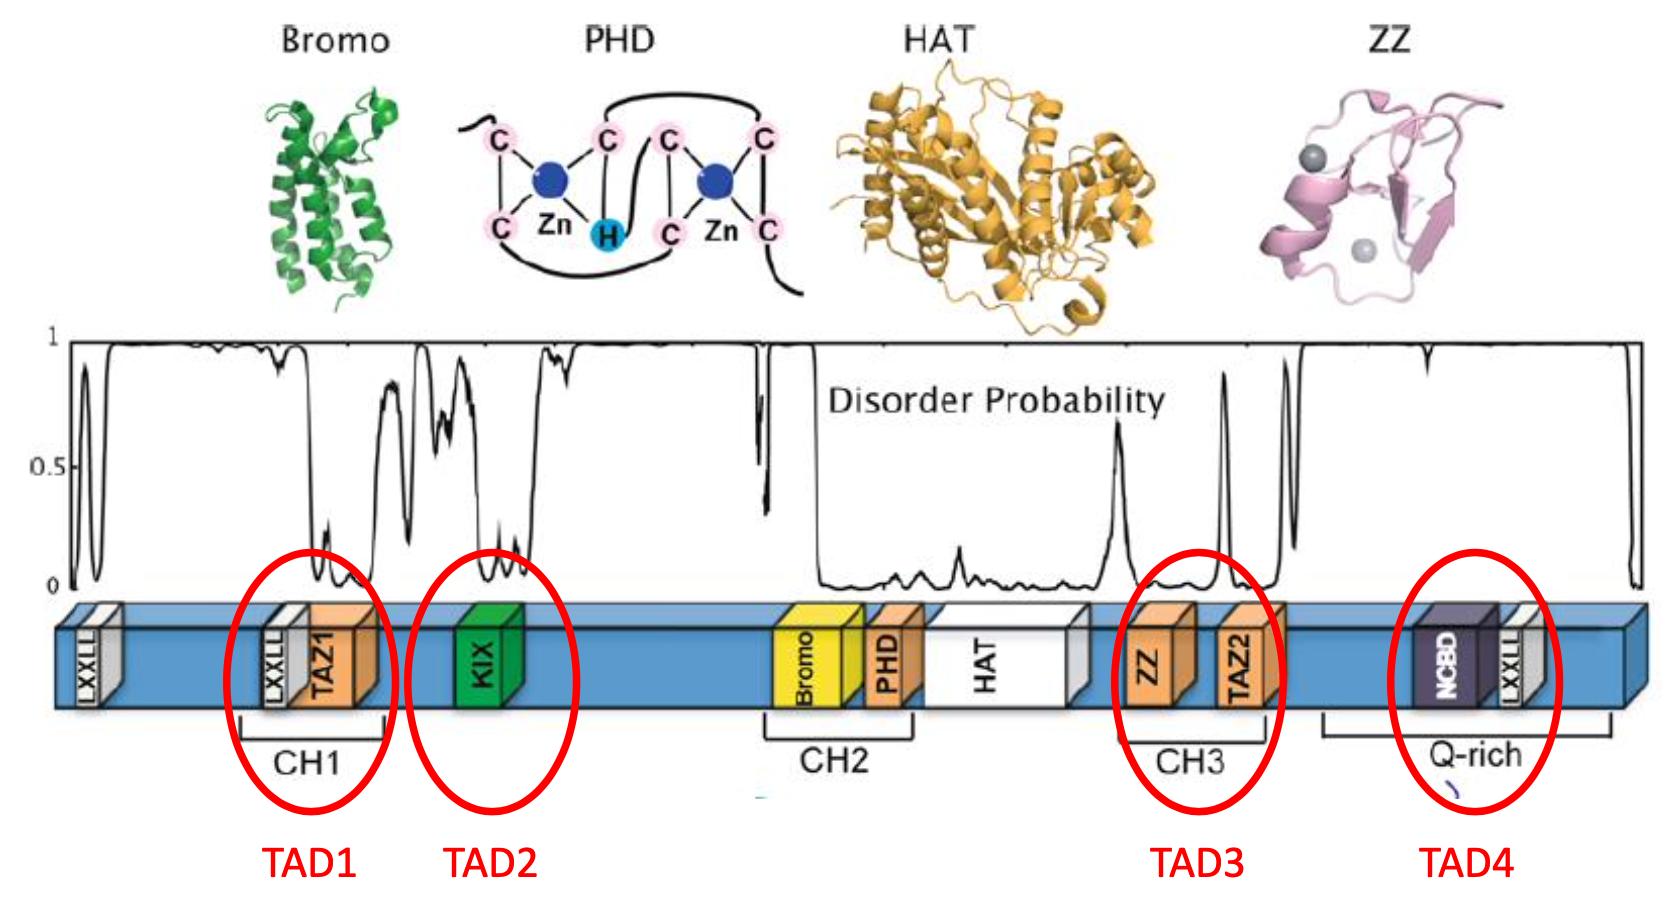
\includegraphics[width=0.5\textwidth]{../_resources/Screenshot_2022-10-12_at_08-56-06.png}
  \caption{Wang \emph{et al., Cell Mol Life Sci.} 2013}
  \end{figure}

  Wang \emph{et al., Cell Mol Life Sci.} 2013
\end{itemize}

There are no intrinsically disordered regions, they fold after interacting with id proteins.

Note that among CBP/p300 binding partners we find both oncosuppressor genes and oncogenes, as well as co-factors.

TF interactions are mediated by TADs. There is a combined interaction among multiple TFs and CBP, enabling the integration of the function of several TFs. The interaction with enhancers does not necessarily correlate with transcription activation; only when the appropriate number and identity is recruited on the enhancer, it becomes functional.

CBP/p300 levels in cells are limiting and different genomic sites or pathways compete for their activity.

In the case of p300, we observe the \emph{co-binding mechanism} with common cofactors or common complexes (transcriptional synergy).

Co-activators facilitate transcription by numerous mechanisms:

\begin{itemize}
\tightlist
\item
  Adaptors function: bridging TFs to the PIC, recruitment of polII to core promoters, recruitment of chromatin remodelling and modifying enzymes to core promoters
\item
  Scaffolding function: facilitating protein-protein and protein-DNA interactions, promoting/stabilizing PIC formation
\item
  Enzymatic activities: Kinase (mediator), KAT (CBP/p300) targeting histones, TFs and non-TF proteins (acetylation of P-TEFb enhances its activity).
\end{itemize}

Their activity can vary from gene to gene depending on TF involved and regulated by PTMs and chromatin accessibility.

In particular, CBP/p300 can regulate pro-proliferative pathways, e.g., cell cycle regulation.

\begin{figure}
\centering
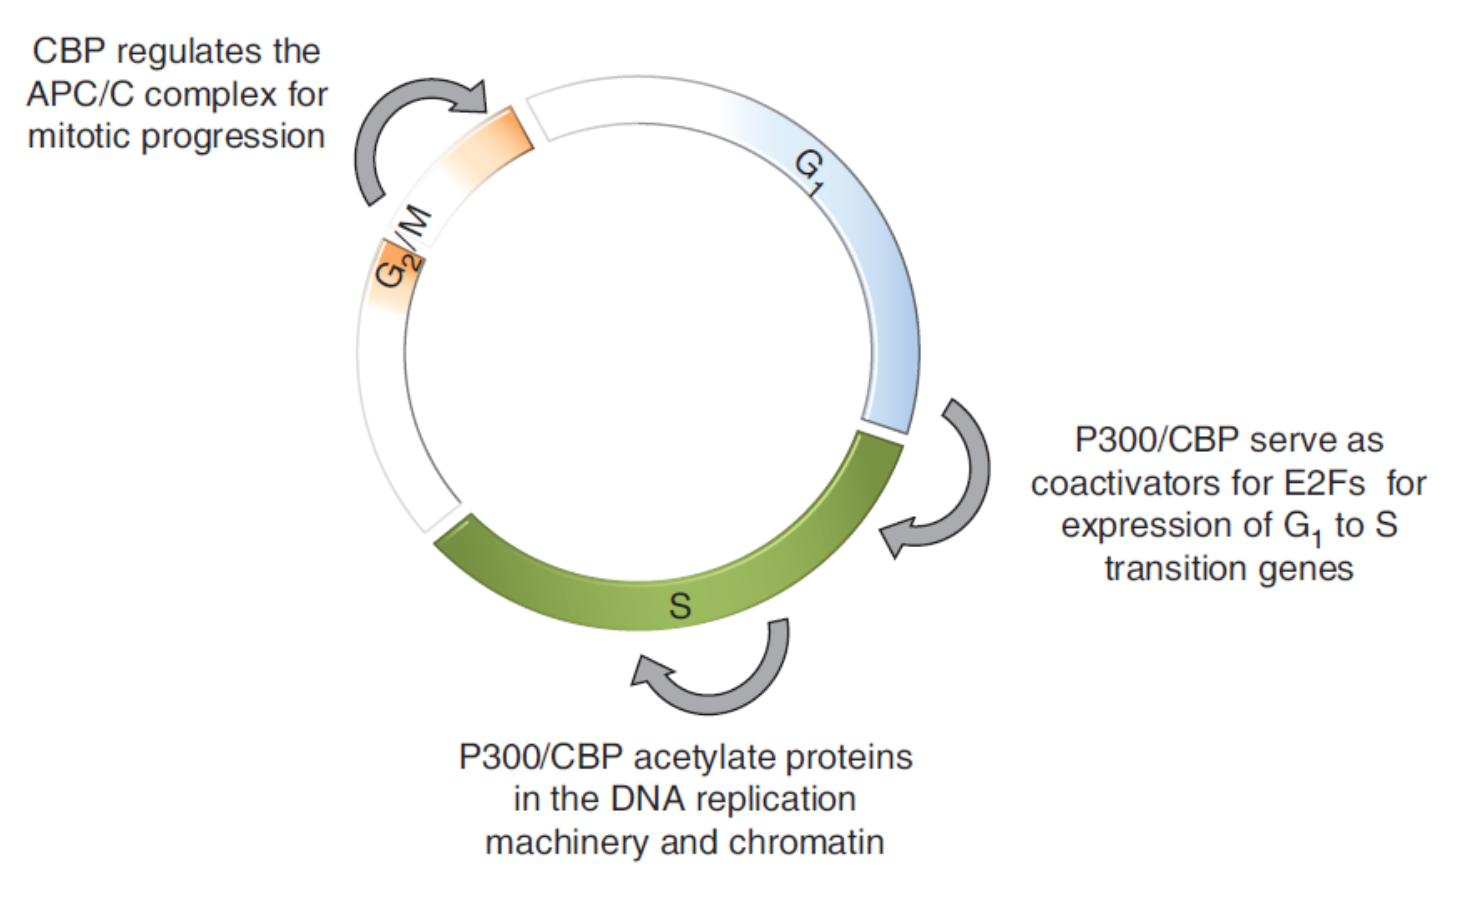
\includegraphics[width=0.5\textwidth]{../_resources/Screenshot_2022-10-12_at_09-01-27.png}
\caption{Screenshot 2022-10-12 at 09.01.27.png}
\end{figure}

Indeed, CBP and p300 gene are frequently mutated in cancer - mutually exclusive. Most are missense mutations (single nucleotide), some deletions and insertions. Mutation hotspots are found at the catalytic domain (KAT). We always need to consider the context of genetic instability characterizing cancer: depending on which signal is activated/repressed, a particular mutated form can either excerpt proliferative or oncosuppressor activity {[}often loss of heterozygosity{]}.

The many functions of CBP/p300 can be differentially exploited in cancer depending on the context, leading the CBP/p300 proteins to act as oncosuppressors or oncogenes. Depending on cellular identity, dysregulated pathways and transcription rewiring, cancer cells may select for the CBP/p300 alterations most advantageous for survival and growth.

\hypertarget{tssa-rnas-transcription}{%
\subsection{\texorpdfstring{\textbf{TSSa-RNAs transcription}}{TSSa-RNAs transcription}}\label{tssa-rnas-transcription}}

Transcription by RNA Pol II is often thought to occur unidirectionally, however we also observe an enrichment of transcripts in the opposite direction with respect to forward transcription. TSSa-RNAs (TSS antisense) surround promoters in nonrandom and divergent orientations. Sense TSSa-RNAs map downstream of the associated promoter, overlapping genic transcripts and peaking in abundance between +0 and +50 nt downstream of the TSS. Antisense TSSa-RNAs peak between nucleotides --100 and --300 and can range from 20 to 90 nt (detected by Northern blot). The mere fact of having high abundance of TF can recruit pol II, which can act \emph{spuriously}: it not only transcribes following the functional direction, but also in the opposite direction (with different pre-initiation complexes).

It is presumed that these small transcripts are abortive transcription tentative; stalling can occur if RNA is not properly processed e.g.~no recruitment of cap proteins, so after degradation and when RNA pol II is displaced, a short sequence (which was protected by pol II) remains at the site. In general, there is a bias towards the directionality of these transcripts, confirming the previous hypothesis; highly expressed genes all have TSSa-RNA.

Although divergent transcription initiation is widespread and might have functions, productive elongation by RNAP II occurs primarily unidirectionally, downstream of TSSs. Promoter upstream transcripts (PROMPTs) are longer than TSS-a and are more stable, while PASRs overlap on the TSS.

Different families of noncoding RNAs are transcribed at promoters of protein coding genes:

\begin{itemize}
\tightlist
\item
  Transcription start-site-associated (\textbf{TSSa}) RNAs are short transcripts (18-24 up to 90bp), do not overlap TSS, sense or antisense of the mRNA
\item
  Promoter associated short transcripts (\textbf{PASRs}): capped bidirectional short RNA (20- 100nt long) that overlap TSS
\item
  Promoter upstream transcripts (\textbf{PROMPTs}): capped bidirectional ncRNAs, map upstream of active promoters (-500 and -2000 from TSS)
\end{itemize}

Potential functions
\begin{itemize}
\item Help modulating chromatin structure due to the Pol II activity and/or binding with chromatin i.e.~help sustaining nucleosome free regions
\item  Noncoding RNAs as precursors for short ncRNA (especially longer ones)
\end{itemize}

{[}RNAse are degraded by the exosome, which is a multi-subunit complex which recognizes uncut RNAse.{]}

\textbf{ENCODE} (Encyclopedia of DNA Elements) has the objective to map all RNAs, which are divided into long and short and by cellular location - either cytoplasmatic or nuclear.

\begin{itemize}
\tightlist
\item
  74.7\% of human genome is transcribed (primary transcripts)
\item
  short RNAs detected:$\sim$160,000 transcripts ( $\sim$40,000 exonic, $\sim$55,000 intronic,$\sim$45,000 intergenic,$\sim$23,000 gene-intergene boundaries)
\item
  long RNA transcripts detected:$\sim$60,000 transcripts from$\sim$19,000 protein coding genes (GENECODE v7); 73,325 transcripts mapping within intergenic regions (also enhancers) and antisense elements (long noncoding RNAs and possible new genes)
\end{itemize}

TSS identified within enhancer regions with transcription proceeding for several kilobases giving rise to \textbf{eRNAs}.

\emph{How can we distinguish enhancers?} By analysing epigenetic marks, TF binding and especially co-factor binding (ChIP-Seq).

Poly(A)- mostly enriched, but also Poly(A), detectable by CAGE hence capped. Transcribed enhancers on average show a significantly different pattern of chromatin modification than non-transcribed ones e.g.~H3K27ac,\ldots{} All the markers are associated with transcription initiations.

In addition to the fact that enhancers need to regulate transcription to allow RNA production, transcription can occur bidirectionally and the enhancer itself can be transcribed.

\begin{itemize}
\tightlist
\item
  \textbf{poised enhancer:} TF bound to the enhancer LDTF (lineage-determinant TF), which is a pioneer TF. We can see some histone modifications for activation, but they are not sufficient to fully activate the promoter. Even pol II can or cannot be recruited, it is not yet acting on a target promoter, but it is active.
\item
  \textbf{active enhancer:} Mediator recruitment, HAT activity, nucleosome remodelling complexes and transcription occurs on the enhancer.
\end{itemize}

Example: the signalling of NFKB TF starts in cytoplasm, it only is shuttled to nucleosome upon a specific signal. Since it is not pioneer TF, it can only bind to poised enhancer → cell-line dependent mechanism.

An active enhancer shows high levels for H3K4me (especially me3), Pol II and Ser5P, H3K27ac, while other elongation markers are less observed. Example of cell-specific regulation: TAL1 TF , oncogene expressed in endothelial cells and erythroid cells, we witness enrichment of H3k4me2 at enhancer sites. Active enhancers associate with chromatin looping.

\hypertarget{properties-of-ernas}{%
\subsubsection{Properties of eRNAs}\label{properties-of-ernas}}

\begin{itemize}
\tightlist
\item
  eRNAs are transcribed from putative enhancer regions characterized by high levels of H3K27ac and the lack of the repressive H3K27me3 mark
\item
  These genomic regions are bound by TFs and associate with transcriptional co- regulators including Mediator, histone acetyltransferase CBP/p300
\item
  eRNA-expressing enhancers are also enriched with PIC
\item
  eRNAs are 50-2000 nt in length and generally exhibit shorter half-lives compared to
  mRNAs and lncRNAs. They are generally not spliced or polyadenylated
\item
  Enhancer transcripts are preferentially enriched at enhancers engaged in chromatin looping with promoters of protein-coding genes and other enhancers, which is a feature correlated with enhancer activity
\end{itemize}

\textbf{eRNAs proposed functions:}

\begin{figure}
\centering
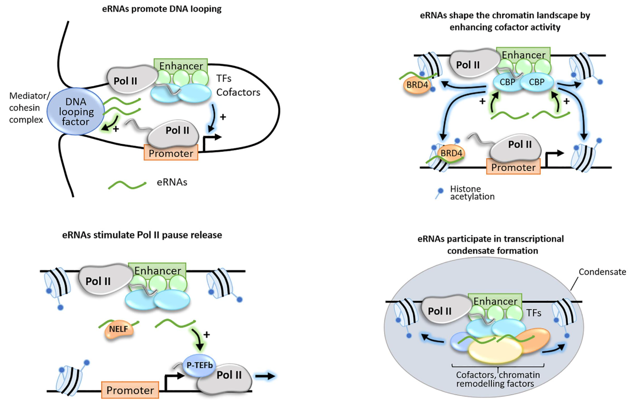
\includegraphics[width=0.5\textwidth]{../_resources/Screenshot_2022-10-12_at_10-00-02.png}
\caption{Studniarek \emph{et al., Trends in Genetics,} 2021}
\end{figure}

Studniarek \emph{et al., Trends in Genetics,} 2021

Last function: Intrinsically disordered proteins → phase separation mechanism. We are enriching the density of enzymes in a particular region.

In particular, eRNA can promoter chromatin remodelling recruitment to reach appropriate configurations for chromatin at TSS.

\hypertarget{assessing-whether-the-crc-8q24-risk-region-acts-as-an-enhancer}{%
\subsubsection{\texorpdfstring{\textbf{Assessing whether the CRC 8q24 risk region acts as an enhancer}}{Assessing whether the CRC 8q24 risk region acts as an enhancer}}\label{assessing-whether-the-crc-8q24-risk-region-acts-as-an-enhancer}}

Most mutations in cancer are SNPs and mainly occur outside of coding regions. Driver mutations are commonly found at coding regions, but also outside of it. One way in which we can analyze non-coding region is assessing the frequency of mutation for a region. In 2007, two different studies found that some SNPs located in 8q24 were highly associated with colorectal cancer.

In particular, the rs6983267 SNP G allele (over T allele) on 8q24 associates with increased risk of colorectal cancer. Homozygosity for the risk G allele in cancer increases CRC risk 1.5 folds.

One way to study non-coding SNP is to understand whether it can be a regulatory region:

\begin{enumerate}
\def\labelenumi{\arabic{enumi}.}
\tightlist
\item
  ChIP-Seq: the risk locus with G shows an enrichment in RNAP II, methylation and p300
\item
  Reporter assay: 1.5 kb long region including the risk allele can function as an enhancer. The G risk allele shows increase reporter activity than the WT allele for the risk allele. It is not a 10 fold difference, suggesting it is not a driver mutation.
\end{enumerate}

Epigenetic and reporter assay data indicate that the CRC risk allele functions as an enhancer.
The rs6983267 SNP is located with a \textbf{TCF} consensus binding site (A/T)(A/T)CAA(A/T)GG. This site is not an exact consensus sequence, but if we have a G on the last position we achieve a higher affinity. By performing ChIP on TCF4, the peak for G allele is higher than T. There is no gene for hundreds of kbs, but if we move forward we find Myc. Since TCF4 is an effector of Wnt pathway and Myc is a beta-catenin target, the SNP can be placed in Myc enhancer region. Instead, no association between MYC mRNA expression and CRC risk allele was identified in either normal colon or tumor samples. However, 3C experiments show a physical interaction between the risk allele and MYC promoter was detected in CRC lines but not fibroblasts.

Conclusions:

\begin{itemize}
\tightlist
\item
  The CRC risk locus shows enhancer-like functions in CRC cell lines
\item
  The CRC risk allele interacts with TCF4
\item
  This locus physically interacts with the MYC promoter
\end{itemize}

Hypothesis: the rs6983267 risk allele may regulate MYC during tumorigenesis

Another article from 2009:

Computational approach predicts that the rs6983267 would impact TCF4 binding site, since a change from T to G is predicted to considerably increase the affinity for TCF4 binding. They use a different approach to verify whether TCF4 is interacting with the risk region.

EMSA: in vitro incubation of recombinant proteins (oligonucleotide of interest with radioactive mark). Run electrophoresis: TCF4 with its own sequence, unrelated sequence and SNP alleles sequence. TCF4 can bind the risk allele G, much less affinity for T allele.

Activation of the WNT pathway through GSK3B inhibition indicates WNT responsive enhancer activity. Reporter assay to obtain a biological readout of the process: the entire site is required for the interaction and should not be further mutated. The risk G allele shows 1.5 fold increase in WNT responsitivity compared to the T allele.
